\documentclass[main.tex]{subfiles}
\begin{document}
\begin{enumerate}

\subsection*{Section 8: Electrical Power \& Energy}

\item[22.] \textbf{Q.} A three-phase 250MVA, 20kV, 60Hz salient pole synchronous machine has parameters $Xd = 1.1$ pu, $Xq = 0.6$ pu and $\operatorname{Ra} \sim 0$. The machine delivers 230MW at 0.9 lagging power factor to an infinite busbar. Calculate the excitation voltage and power angle. Draw the phasor diagram. (Hint: use per unit values and give your answers in pu). 

\textbf{Theory.} A Salient Pole Synchronous Generator, is distinguished from a round rotor machine by constructional features of field poles which project with a large interpolar air gap. This type of construction is commonly employed in machines coupled to hydroelectric turbines which are inherently slow-speed ones so that the Salient Pole Synchronous Generator has multiple pole pairs as different from machines coupled to high-speed steam turbines (3,000/1,500 rpm) which have a two- or four-pole structure. Salient Pole Synchronous Generator analysis is made through the two-reaction theory. In a salient-pole rotor synchronous machine, the air-gap is highly non-uniform. Consider a synchronous machine having a 2-pole salient-pole rotor rotating in the anti-clockwise direction within a 2-pole stator, as shown in Figure \ref{fig:22a_a}. 

\begin{figure}
\centering\fbox{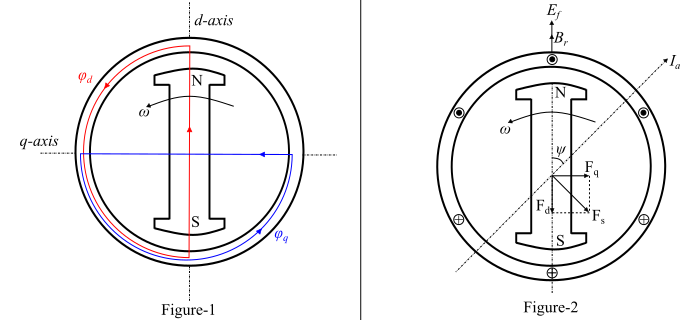
\includegraphics[width=4.0in]{2018spring/figures/22a_a.png}}
\caption{Salient Pole Synchronous Generator}
\label{fig:22a_a}
\end{figure}

In Figure \ref{fig:22a_a}, the axis shown along the axis of the rotor is known as direct axis or $d$-axis and the axis perpendicular to the $d$-axis is called quadrature axis or q-axis. It can be seen that the two small air-gaps are involved in the path of $d$ axis flux $\left(\varphi_d\right)$, thus the reluctance of the path is minimum. The q-axis flux $\left(\varphi_q\right)$ path has two large air-gaps and it is the path of maximum reluctance. The rotor magnetic field $\left(\boldsymbol{B}_r\right)$ is shown directed vertically upward in Figure \ref{fig:22a_a}. This rotor magnetic field induces an EMF in the armature (or stator winding). If a lagging power factor load is connected to the alternator, an armature current $\left(\boldsymbol{I}_{\boldsymbol{a}}\right)$ will flow. The armature current $\left(\boldsymbol{I}_a\right)$ lags behind the excitation voltage $\left(\boldsymbol{E}_f\right)$ by an angle $\Psi$ (see Figure \ref{fig:22a_a}). The armature current $\left(\boldsymbol{I}_a\right)$ produces the stator MMF $\left(F_S\right)$ which lags behind $\boldsymbol{I}_{\boldsymbol{a}}$ by $90^{\circ}$. The stator MMF $\left(F_s\right)$ produces the stator magnetic field $\left(\boldsymbol{B}_s\right)$ along the direction of $F_S$. According to Blondel's Two Reaction Theory, the stator MMF $\left(F_S\right)$ can be resolved into two components viz. the direct axis component $\left(F_d\right)$ and the quadrature axis component $\left(F_q\right)$. If $\varphi_d=$ Direct axis flux, $\varphi_q=$ Quadrature axis flux, $S_d=$ Reluctance of direct axis flux path and $S_q=$ Reluctance of quadrature axis flux path, then the Direct axis flux is

$$
\varphi_d=\frac{F_d}{S_d}
$$

and the Qaudrature axis flux is

$$
\varphi_q=\frac{F_q}{S_q}.
$$

Since $S_d<S_q$, the direct axis component $\left(F_d\right)$ of stator MMF produces more flux than the quadrature axis component $\left(F_q\right)$ of the stator MMF. The direct axis and quadrature axis components of the stator fluxes produce voltages in the stator winding by armature reaction. Let, $\boldsymbol{E}_{a d}=$ Direct axis component of armature reaction voltage and $\boldsymbol{E}_{a q}=$ Quadrature axis component of armature reaction voltage. Since each armature reaction voltage is directly proportional to respective armature current and lags behind the armature current by $90^{\circ}$, the armature reaction voltages can be written as,

$$
\boldsymbol{E}_{a d}=-j \boldsymbol{I}_d X_{a d} 
$$

$$
\boldsymbol{E}_{a q}=-j \boldsymbol{I}_q X_{a q} 
$$

Where, $\because X_{a d}$ is the armature reaction reactance in the direct axis per phase.
$X_{a q}$ is the armature reaction reactance in the quadrature axis per phase.
Here, $X_{a q}<X_{a d}$ because the EMF induced by a given MMF acting on the direct axis is smaller than the EMF on the quadrature axis due to its higher reluctance.
Now, the resultant EMF induced in the machine is,

$$
\boldsymbol{E}_R=\boldsymbol{E}_f+\boldsymbol{E}_{a d}+\boldsymbol{E}_{a q}
$$

$$
\Rightarrow \boldsymbol{E}_R=\boldsymbol{E}_f-j \boldsymbol{I}_d X_{a d}-j \boldsymbol{I}_q X_{a q}
$$

Also, the resultant voltage $\left(\boldsymbol{E}_R\right)$ is equal to the phasor sum of terminal voltage and the voltage drops in the resistance and leakage reactance of the armature, thus,

$$
\boldsymbol{E}_R=\boldsymbol{V}+\boldsymbol{I}_a \boldsymbol{R}_a+j \boldsymbol{I}_a X_l
$$

The armature current $\left(\boldsymbol{I}_a\right)$ is split into two components, one in phase with the excitation voltage $\left(\boldsymbol{E}_f\right)$ and the other in phase quadrature to it.
If $\boldsymbol{I}_q=$ quadrature axis component of $\boldsymbol{I}_a$ in phase with $\boldsymbol{E}_f$, $\boldsymbol{I}_d=$ direct axis component of $\boldsymbol{I}_a$ lagging $\boldsymbol{E}_f$ by $90^{\circ}$. Then, the total armature current is the phasor sum of $\boldsymbol{I}_q$ and $\boldsymbol{I}_d$, i.e.,

$$
\boldsymbol{I}_a=\boldsymbol{I}_q+\boldsymbol{I}_d
$$

Now, from equations we get,

$$
\boldsymbol{E}_f=\boldsymbol{V}+\boldsymbol{I}_a \boldsymbol{R}_a+j \boldsymbol{I}_a X_l+j \boldsymbol{I}_d X_{ad}+j \boldsymbol{I}_q X_{aq} 
$$

And, from equations we get,

$$
\begin{aligned}
\boldsymbol{E}_f&=\boldsymbol{V}+\left(\boldsymbol{I}_q+\boldsymbol{I}_d\right) \boldsymbol{R}_a+j\left(\boldsymbol{I}_q+\boldsymbol{I}_d\right) X_l+j \boldsymbol{I}_d X_{a d}+j \boldsymbol{I}_q X_{a q}\\
&=\boldsymbol{V}+\left(\boldsymbol{I}_q+\boldsymbol{I}_d\right) \boldsymbol{R}_a+j \boldsymbol{I}_d\left(X_l+X_{a d}\right)+j \boldsymbol{I}_q\left(X_l+X_{a q}\right)\\
&=\boldsymbol{V}+\left(\boldsymbol{I}_q+\boldsymbol{I}_d\right) \boldsymbol{R}_a+j \boldsymbol{I}_d X_d+j \boldsymbol{I}_q X_q
\end{aligned}
$$

Where,

$$
X_d=X_l+X_{a d} \quad \text { and } \quad X_q=X_l+X_{a q}
$$

The reactance $X_d$ is known as the direct-axis synchronous reactance and the reactance $X_q$ is called the quadrature-axis synchronous reactance.

$$
\therefore \boldsymbol{E}_f=\boldsymbol{V}+\boldsymbol{I}_a \boldsymbol{R}_a+j \boldsymbol{I}_d X_d+j \boldsymbol{I}_q X_q
$$

The final form of the voltage equation for a salient-pole synchronous generator. Reference Figure \ref{fig:22a_b} for the phasor diagram.

\begin{figure}
\centering\fbox{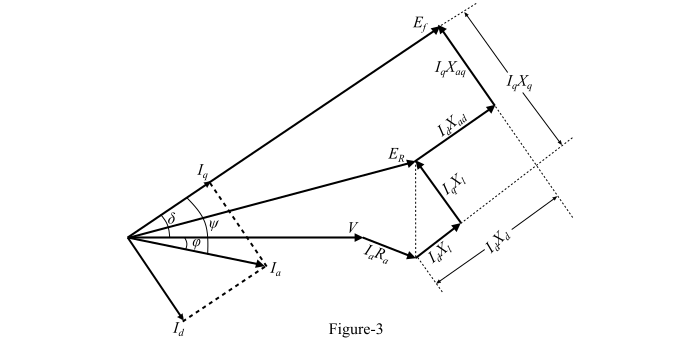
\includegraphics[width=5.0in]{2018spring/figures/22a_b.png}}
\caption{The complete phasor diagram of a salient-pole synchronous generator based on the Blondel’s Two Reaction Theory.}
\label{fig:22a_b}
\end{figure}

\textbf{A.} Given that the machine delivers $230 \mathrm{MW}$ at 0.9 lagging power factor to an infinite busbar, we can calculate the apparent power $\mathrm{S}$ as follows:

$$
S=\frac{P}{p f}=\frac{230 M W}{0.9}=255.56 M V A
$$

Since the machine is rated at 250MVA, we can convert the apparent power to per unit (pu) as follows:

$$
S_{p u}=\frac{S}{S_{\text {base }}}=\frac{255.56 \mathrm{MVA}}{250 \mathrm{MVA}}=1.022 p u
$$

The current I can be calculated as follows:

$$
I=\frac{J}{V}=\frac{\angle \supset J . J 0 M V A}{20 k V}=12.778 \mathrm{kA}
$$

Since the power factor is lagging, the current I lags the voltage $\mathrm{V}$ by an angle of $\cos ^{\wedge}-1(0.9)=25.84^{\circ}$. We can represent the current $I$ in rectangular form as follows:

$$
I=12.778 k A \angle-25.84^{\circ}=11.5 k A-j 4.5 k A
$$

Converting the current to pu, we get:

$$
I_{p u}=\frac{I}{I_{\text {base }}}=\frac{12.778 \mathrm{kA}}{12.5 \mathrm{kA}}=1.022 p u \angle-25.84^{\circ}=0.92 p u-j 0.36 p u
$$

Since $\mathrm{Ra} \sim 0$, we can ignore the armature resistance and calculate the internal voltage $\mathrm{E}$ as follows:

$$
\begin{gathered}
E=V+j X q I q+j X d I d \\
E=V+j X q I \sin (\theta)+j X d I V \cos (\theta)
\end{gathered}
$$

where $\mathrm{V}$ is the terminal voltage, $\mathbf{X q}$ and $\mathbf{X d}$ are the quadrature-axis and direct-axis reactances respectively, and $I$ and $\theta$ are the magnitude and angle of the current respectively.
Substituting the given values, we get:

$$
\begin{gathered}
E=1+j 0.6(1.022)(-0.36)+j 1.1(1.022)(0.92) \\
E=1+j(-0.221)+j 1.1242 \\
E=1+j 0.9032 p u
\end{gathered}
$$

The power angle $\delta$ can be calculated as follows:

$$
\delta=\tan ^{-1}\left(\frac{\operatorname{Im}(E)}{\operatorname{Re}(E)}\right)=\tan ^{-1}\left(\frac{0.9032}{1}\right)=41.99^{\circ}
$$

\item[23.] \textbf{Q.} A wind turbine is to be designed with an electrical power output of 7.0MW. The rated upwind free wind speed is 13 m/s. Determine the length of the rotor blades and the height of the supporting tower in meters and the rotational speed of the rotor in rev/min if the tip-speed ratio whose value as 7.0 determines the maximum Power Coefficient of 0.45. Use the density of air as $\num{1.225}\unit{kg/m^3}$. \textbf{A.} The power output of a wind turbine can be calculated using the formula: 

$$
P=\frac{1}{2} \rho A C_p v^3
$$

where $\rho$ is the density of air, $A$ is the swept area of the rotor, $C_p$ is the power coefficient, and $v$ is the wind speed. Given: $P =4 \mathrm{MW}=4 \times 10^6 \mathrm{~W}$, $\rho = 1.225 \unit{kg/m^3}$ $C_p=0.45$, $v = 13 \mathrm{m} / \mathrm{s}$. Calculate area swept by the blades 

$$
\begin{aligned}
4 \times 10^6 & =\frac{1}{2} \times 1.225 \times A \times 0.45 \times (13)^3. \\
A &= 6,605.59 \mathrm{~m}^2
\end{aligned}
$$

Area $=\pi r^2$ where $r=$ length of the blades

$$
\begin{aligned}
6,605.59 \mathrm{~m}^2 &= \pi r^2 \\
r^2 &= \frac{6,605.59}{\pi}\mathrm{~m}^2\\
r &= \frac{81.2748}{\sqrt{\pi}} \mathrm{~m}\\
&= 45.8544 \mathrm{~m}
\end{aligned}
$$

Current design standards set a fixed rate of 1-1.3 for the height to diameter ratio as this is the estimated best ratio to receive the most power output for the least cost. The tip speed ratio is defined as

$$
\lambda = \frac{\text{Tip speed of Blade}}{\text{Wind Speed}} =  \frac{2 \pi r N}{v}
$$

where $N=$ speed in rps (revolutions per second), $r=$ length of the blade, and $v=$ free wind velocity. Calculate revolutions per minute

$$
\begin{aligned}
7 &= \frac{2 \pi \times 45.8 \times N}{13} \\ 
N &= \frac{7 \times 13}{2 \pi \times 45.8}\\
&= 0.32 \mathrm{~rps}\\
&= 0.32 \times 60 = 18.97 \mathrm{~rpm}
\end{aligned}
$$

\item[24.] \textbf{Q.} A 450MVA, 20kV, 60-Hz round-rotor synchronous generator has an Inertia constant H = 5s. Displayed on the axes in Figure \ref{fig:24q_a} are Torque/Angle characteristics for various faults occurring on a double circuit transmission line when connected between a synchronous generator and an infinite busbar. Using the Equal Area Criterion, determine the critical switching times for both a $3 \varphi$ fault and a Line to Line fault when the input and torque from the turbine is 1.0 pu as shown in the diagram. 

\begin{figure}
\centering\fbox{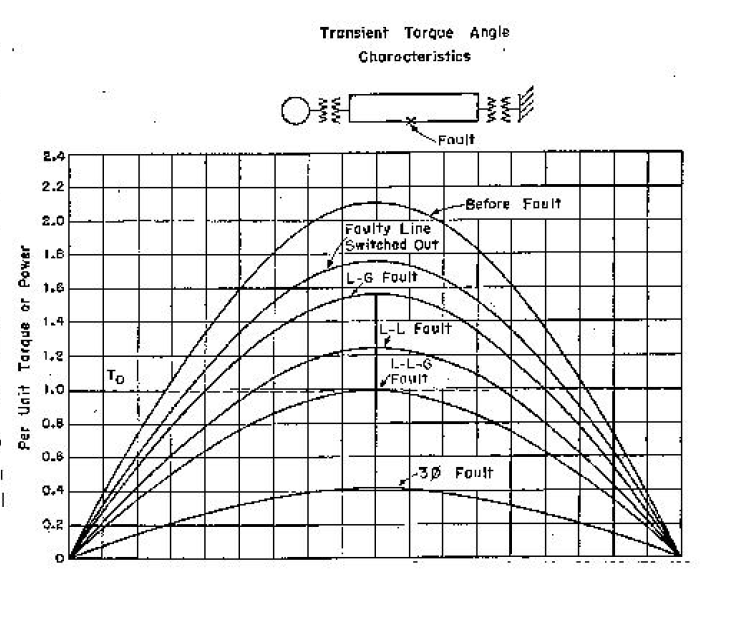
\includegraphics[width=5.0in]{2018spring/figures/24q_a.png}}
\caption{Transient Torque Angle characteristics, per unit torque or power}
\label{fig:24q_a}
\end{figure}

\textbf{Theory.} A single circuit transmission line has three sets of conductors, while a double circuit transmission line is two independent circuits on the same structure with each circuit made up of three sets of conductors. An infinite busbar has a fixed voltage and frequency even after a variation in the load. A synchronous generator is a synchronous machine which converts mechanical power into AC electric power through the process of electromagnetic induction. Synchronous generators are also referred to as alternators or AC generators. The equal area criterion is a simple graphical method for concluding the transient stability of two-machine systems or a single machine against an infinite bus. This principle does not require the swing equation for the determination of stability conditions. The stability conditions are recognized by equating the areas of segments on the power angle diagram between the p-curve and the new power transfer line of the given curve.

\textbf{A.} To determine the critical switching time for a $3 \varphi$ fault, we need to find the intersection point between the "3P Fault" line and the line representing the input torque from the turbine. The area under these two lines represents the kinetic energy stored in the rotor during the fault. The critical switching time is then determined by finding the point at which this area is equal to the area under the "3P Fault" line after the fault has been cleared. In $p-\delta$ plot shown in Figure \ref{fig:24q_a} at the critical clearing angle, denoted $\delta_{\mathrm{cr}}$, the fault is extinguished. The power angle then increases to a maximum value $\delta_{max} =$ which gives the maximum decelerating area. Plots of electrical power $p_e$ and mechanical power $p_m$ versus power angle $\delta$ are shown in Figure \ref{fig:24q_a}. $p_e$ is a sinusoidal function of $\delta$, as given by $p_e = P_{\max } \sin \delta$. Solve for the initial power angle $\delta_0$ and max power angle $\delta_{max} = \pi-\delta_0$ which bound the accelerating and decelerating areas

\begin{figure}
\centering\fbox{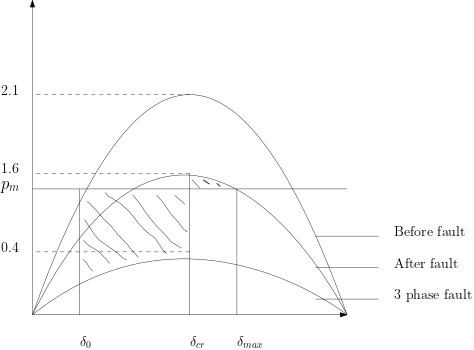
\includegraphics[width=5.0in]{2018spring/figures/24a_a.png}}
\caption{$3 \varphi$ fault Equal Area Criterion}
\label{fig:24a_a}
\end{figure}

$$
\begin{aligned}
p_m &= P_{\max} \sin \delta\\
\delta_0 &= \sin^{-1}\left(\frac{1}{P_{\text{BeforeMax}}}\right)\\
\delta_0 &= \sin^{-1}\left(\frac{1}{2.1}\right)\\
&= 0.4963\\
\delta_{\max} &= \pi - \sin^{-1}\left(\frac{1}{P_{\text{AfterMax}}}\right)\\
\delta_{\max} &= \pi - \sin^{-1}\left(\frac{1}{1.6}\right)\\
&= \pi - 0.6751\\
&= 2.4664
\end{aligned}
$$

Solve for the critical power angle $\delta_{\mathrm{cr}}$ where the fault is extinguished by using the equal area criterion by equating the accelerating and decelerating areas 

$$
\begin{aligned}
\mathrm{A}_1=\int_{\delta_0}^{\delta_{cr}} (p_m - P_{3 \varphi max} \sin \delta) d\delta 
&= \mathrm{A}_2 = \int_{\delta_{cr}}^{\delta_{max}} (P_{cmax} \sin \delta - p_m) d \delta \\
\int_{0.4963}^{\delta_{cr}} (1.0-0.4 \sin \delta) d\delta &= \int_{\delta_{cr}}^{2.4664}(1.6 \sin \delta-1.0) d \delta \\
(\delta_{cr} - 0.4963) - 0.4(-\cos \delta)_{0.4963}^{\delta_{cr}} &= 1.6(-\cos \delta)_{\delta_{c r}}^{2.4664}-\left(2.4664-\delta_{c r}\right) \\
\left(\delta_{cr} - 0.4963\right) - 0.4\left(-\cos \delta_{cr} + 0.8793 \right) &= 1.6\left(0.78 + \cos \delta_{cr}\right) - \left(2.4664-\delta_{cr}\right) \\
-0.4963 + 0.4 \cos \delta_{cr} - 0.3517 &= 1.248 + 1.6 \cos \delta_{cr} - 2.4664 \\
0.3704 &= 1.2 \cos \delta_{c r} \\
\delta_{c r} &= 1.257 \mathrm{~rad}.
\end{aligned}
$$


From the solution to the swing equation 

$$
\delta(t)=\frac{\omega_{\text {syn }} p_{m p . u .}}{4 \mathrm{H}} t^2+\delta_0
$$

solve for $t$

$$
t=\sqrt{\frac{4 \mathrm{H}}{\omega_{\text {syn }} p_{m p . u}}\left(\delta(t)-\delta_0\right)}.
$$

Use $\delta_{cr}$ to calculation the critical time $t_{cr}$ for $\delta=\delta_{c r}$

$$
\begin{aligned}
H &= 5\\
t_{cr} &= \left(\frac{4 H}{2\pi f P_m} \left(\delta_{cr}-\delta_0\right) \right)^{1 / 2} \\
t_{cr} &= \left(\frac{4 \times 5}{2\pi \times 60 \mathrm{~Hz} \times 1} (1.257-0.4963) \right)^{1 / 2} \\
t_{cr} &= 0.2841 \mathrm{~s} 
\end{aligned}
$$

To determine the critical switching time for a Line to Line fault, we need to find the intersection point between the L-L fault line and the line representing the input torque from the turbine. The area under these two lines represents the kinetic energy stored in the rotor during the fault. The critical switching time is then determined by finding the point at which this area is equal to the area under the "L-L Fault" line after the fault has been cleared. Refer to figure \ref{fig:24a_b}.

\begin{figure}
\centering\fbox{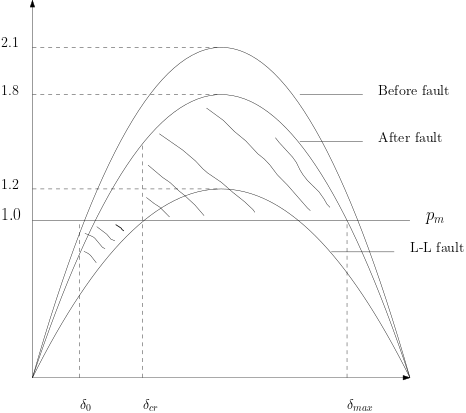
\includegraphics[width=5.0in]{2018spring/figures/24a_b.png}}
\caption{Line to Line fault Equal Area Criterion}
\label{fig:24a_b}
\end{figure}

$$
\begin{aligned}
\delta_0&=0.4963 \text{~rad} \\
\delta_{\mathrm{max}} &= 2.4664 \text{~rad}\\
\mathrm{A}_1=\int_{\delta_0}^{\delta_{cr}} (p_m - P_{LLmax} \sin \delta) d\delta 
&= \mathrm{A}_2 = \int_{\delta_{cr}}^{\delta_{max}} (P_{Cmax} \sin \delta - p_m) d \delta \\
\int_{0.4963}^{\delta_{cr}} (1.0 - 1.2 \sin \delta) d\delta &= \int_{\delta_{cr}}^{2.4664}(1.8 \sin \delta-1.0) d \delta \\
(\delta_{cr} - 0.4963) - 1.2(-\cos \delta)_{0.4963}^{\delta_{cr}} &= 1.8(-\cos \delta)_{\delta_{c r}}^{2.4664}-\left(2.4664-\delta_{c r}\right) \\
\left(\delta_{cr} - 0.4963\right) - 1.2\left(-\cos \delta_{cr} + 0.8793 \right) &= 1.8\left(0.78 + \cos \delta_{cr}\right) - \left(2.4664-\delta_{cr}\right) \\
-0.4963 + 1.2 \cos \delta_{cr} - 1.05516 &= 1.404 + 1.8 \cos \delta_{cr} - 2.4664 \\
-0.4891 &= 0.6 \cos \delta_{c r} \\
\delta_{c r} &= 2.5237 \radian \mathrm{~rad} \\
H &= 5\\
t_{cr} &= \left(\frac{4 H}{2\pi f P_m} \left(\delta_{cr}-\delta_0\right) \right)^{1 / 2} \\
t_{cr} &= \left(\frac{4 \times 5}{2\pi \times 60 \mathrm{~Hz} \times 1} (2.5237-0.4963) \right)^{1 / 2} \\
t_{cr} &= 0.3279 \mathrm{~s} 
\end{aligned}
$$
\end{enumerate}
\end{document}